\section{Raccolta, processing e visualizzazione dei risultati in MATLAB}

\begin{frame}{Wiki DecaWaveEVB1000Experiments}
  Al \href{https://github.com/GiulioRomualdi/DecaWaveEVB1000Experiments/wiki}{\textcolor{blue}{link}} è presente un Wiki che spiega
  come raccogliere dati di Ranging, Autoranging e Trilaterazione utilizzando il software DecaWave EVB1000 Collector sviluppato durante il progetto.\\
  Al medesimo si trovano istruzioni su alcuni script/funzioni MATLAB che consentono di visualizzare i dati e di ottenerne
  ulteriori in postprocessing (ad esempio ottenere la posizione cartesiana delle ancore a partire dai range medi
  raccolti durante l'autoranging oppure la trilaterazione a partire dai range tra tag ed ancore raccolti durante
  un esperimento di trilaterazione).
  Si invita il lettore interessato a consultare tale Wiki.\\
  Di seguito invece si riportano alcuni plot ottenuti utilizzando le istruzioni contenute nel Wiki.
\end{frame}

\begin{frame}{Confronto tra Autoranging, Tag Over Anchor e Laser Meas}
  Nel plot della slide successiva sono mostrate, per ogni range di interesse, le distribuzioni dei range raccolti
  \begin{itemize}
  \item[-] da ogni ancora durante la procedura di autoranging (in azzurro);
  \item[-] posizionando il tag al di sopra di ogni ancora (procedura Tag Over Anchor) (in rosso);
  \item[-] utilizzando un laser range measurer (linea blu tratteggiata).
  \end{itemize}
\end{frame}

\begin{frame}{Confronto tra Autoranging, Tag Over Anchor e Laser Meas}
  \begin{center}
    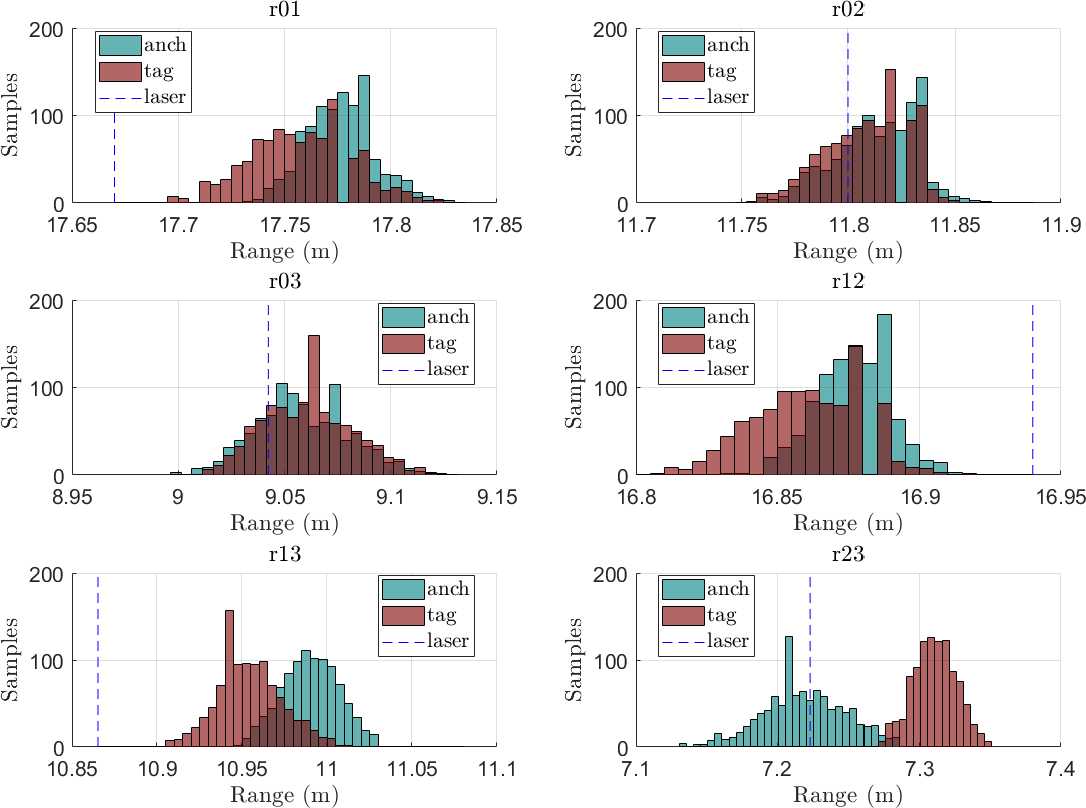
\includegraphics[width=\linewidth]{a2a_histograms.png}
  \end{center}
\end{frame}

\begin{frame}{Raccolta range durante la procedura di autoranging}
  Nei plot delle slide successive vengono mostrate quattro sessioni di raccolta di range durante la procedura di autoranging.
  In ogni sessione vengono raccolte rispettivamente $500$, $5000$, $25000$ e $50000$ misure di range per ogni range di interesse. Viene inoltre mostrato, per confronto, la misura di range effettuata con il sistema di misurazione laser.
\end{frame}

\begin{frame}{Trilaterazione con due tag - Range raccolti: $500$}
  \begin{center}
    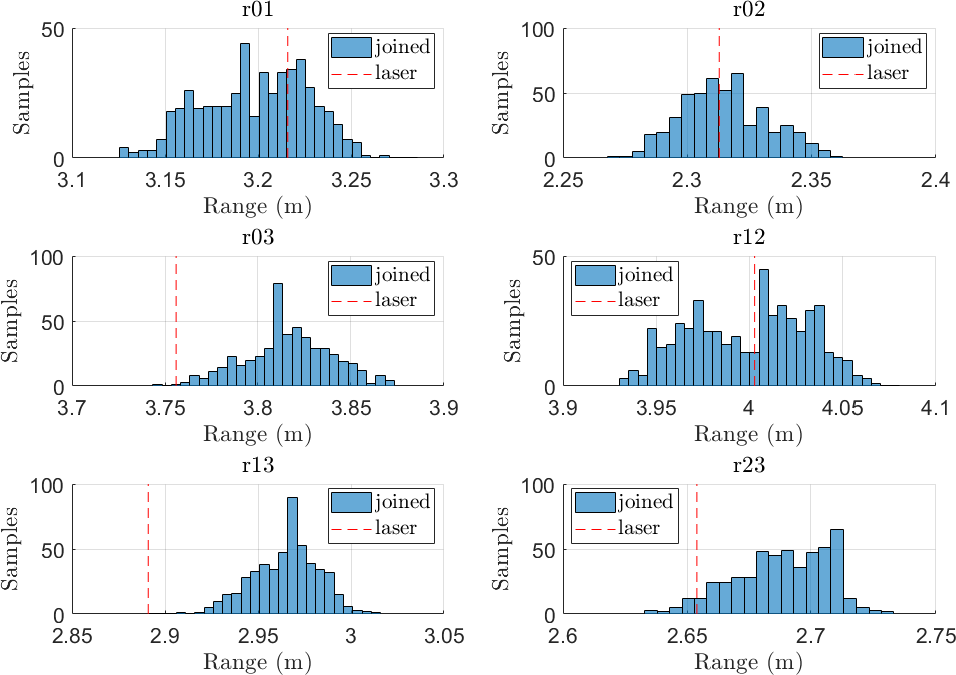
\includegraphics[width=\linewidth]{autoranging_500.png}
  \end{center}
\end{frame}

\begin{frame}{Trilaterazione con due tag - Range raccolti: $5000$}
  \begin{center}
    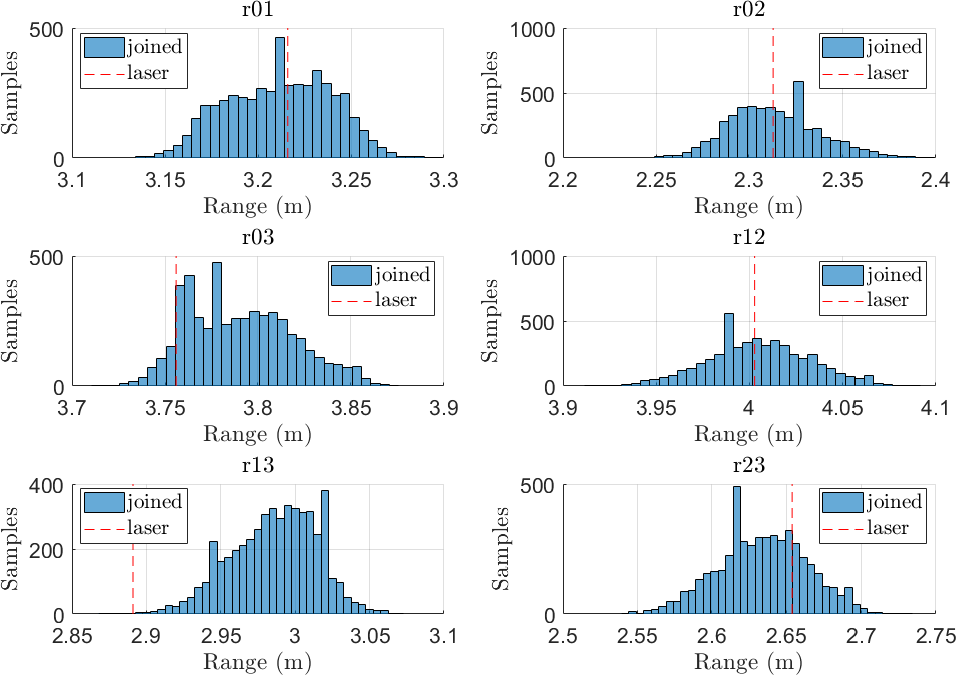
\includegraphics[width=\linewidth]{autoranging_5000.png}
  \end{center}
\end{frame}

\begin{frame}{Trilaterazione con due tag - Range raccolti: $25000$}
  \begin{center}
    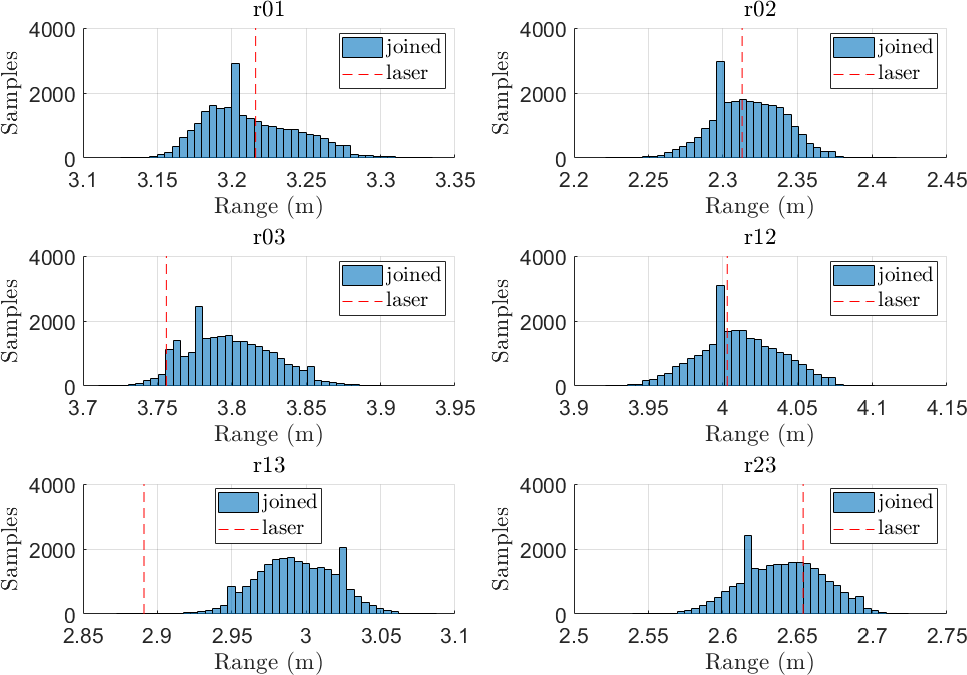
\includegraphics[width=\linewidth]{autoranging_25000.png}
  \end{center}
\end{frame}

\begin{frame}{Trilaterazione con due tag - Range raccolti: $50000$}
  \begin{center}
    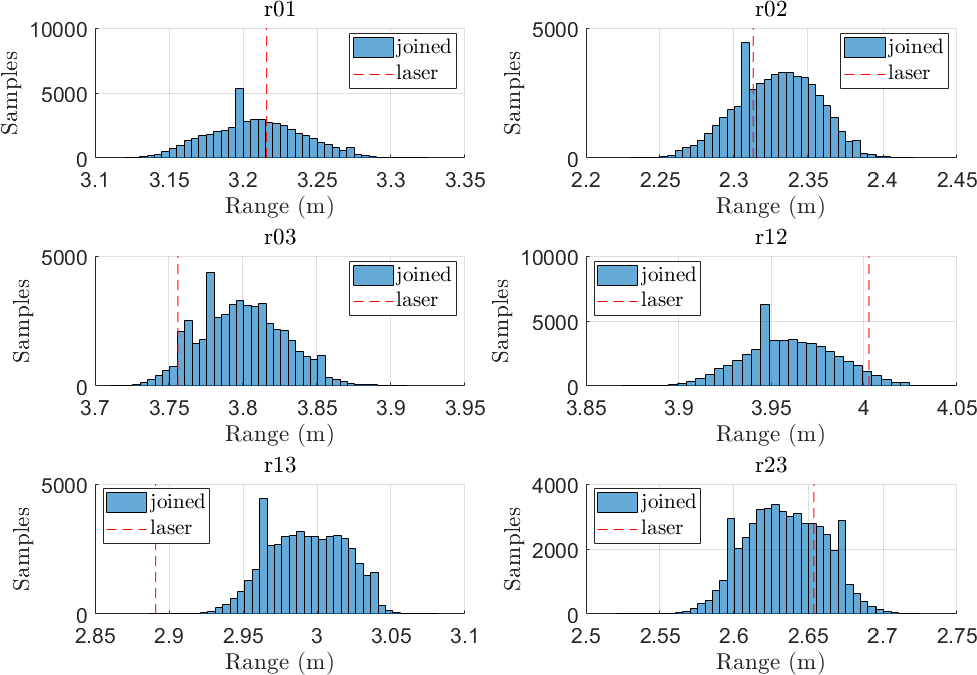
\includegraphics[width=\linewidth]{autoranging_50000.png}
  \end{center}
\end{frame}

\begin{frame}{Trilaterazione: confrontro tra DecaWave, DecaWave Cycle e Algebraic}
  Nel plot della slide successiva è mostrato il risultato della trilaterazione ottenuto
  in postprocessing attraverso gli algoritmi DecaWave, DecaWave Cycle e Algebraic.\\
  Sono state utilizzate le posizioni delle ancore ottenute mediante Autoranging.
\end{frame}

\begin{frame}{Trilaterazione: confrontro tra DecaWave, DecaWave Cycle e Algebraic}
  \begin{center}
    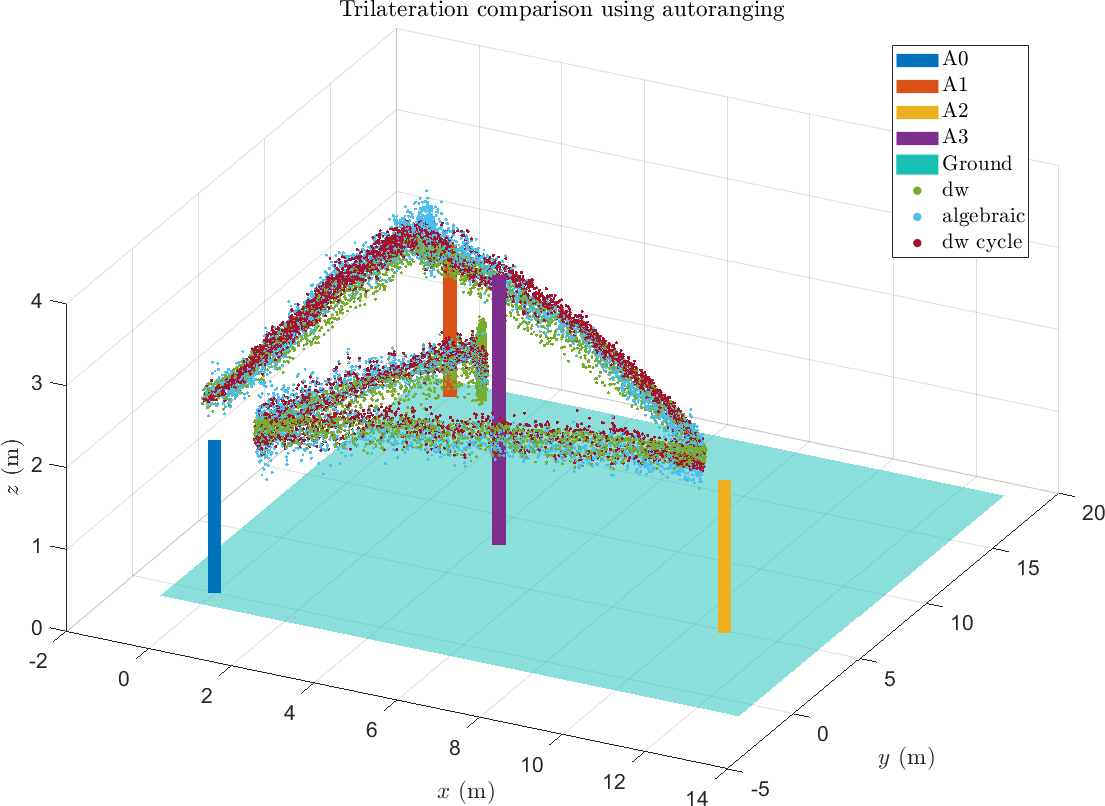
\includegraphics[height=19em]{3d_path.png}
  \end{center}
\end{frame}

\begin{frame}{Trilaterazione: confrontro tra DecaWave, DecaWave Cycle e Algebraic}
  \begin{center}
    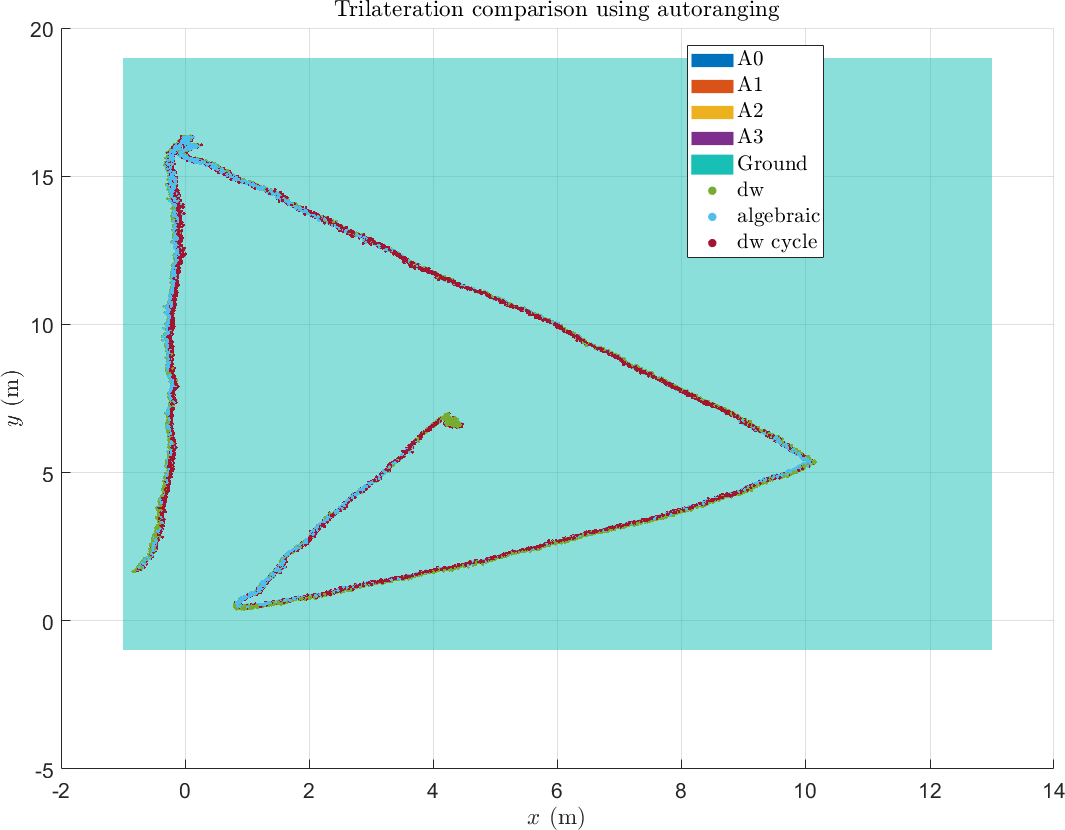
\includegraphics[height=19em]{3d_path_pianta.png}
  \end{center}
\end{frame}

\begin{frame}{Trilaterazione: confrontro tra DecaWave, DecaWave Cycle e Algebraic}
  \begin{center}
    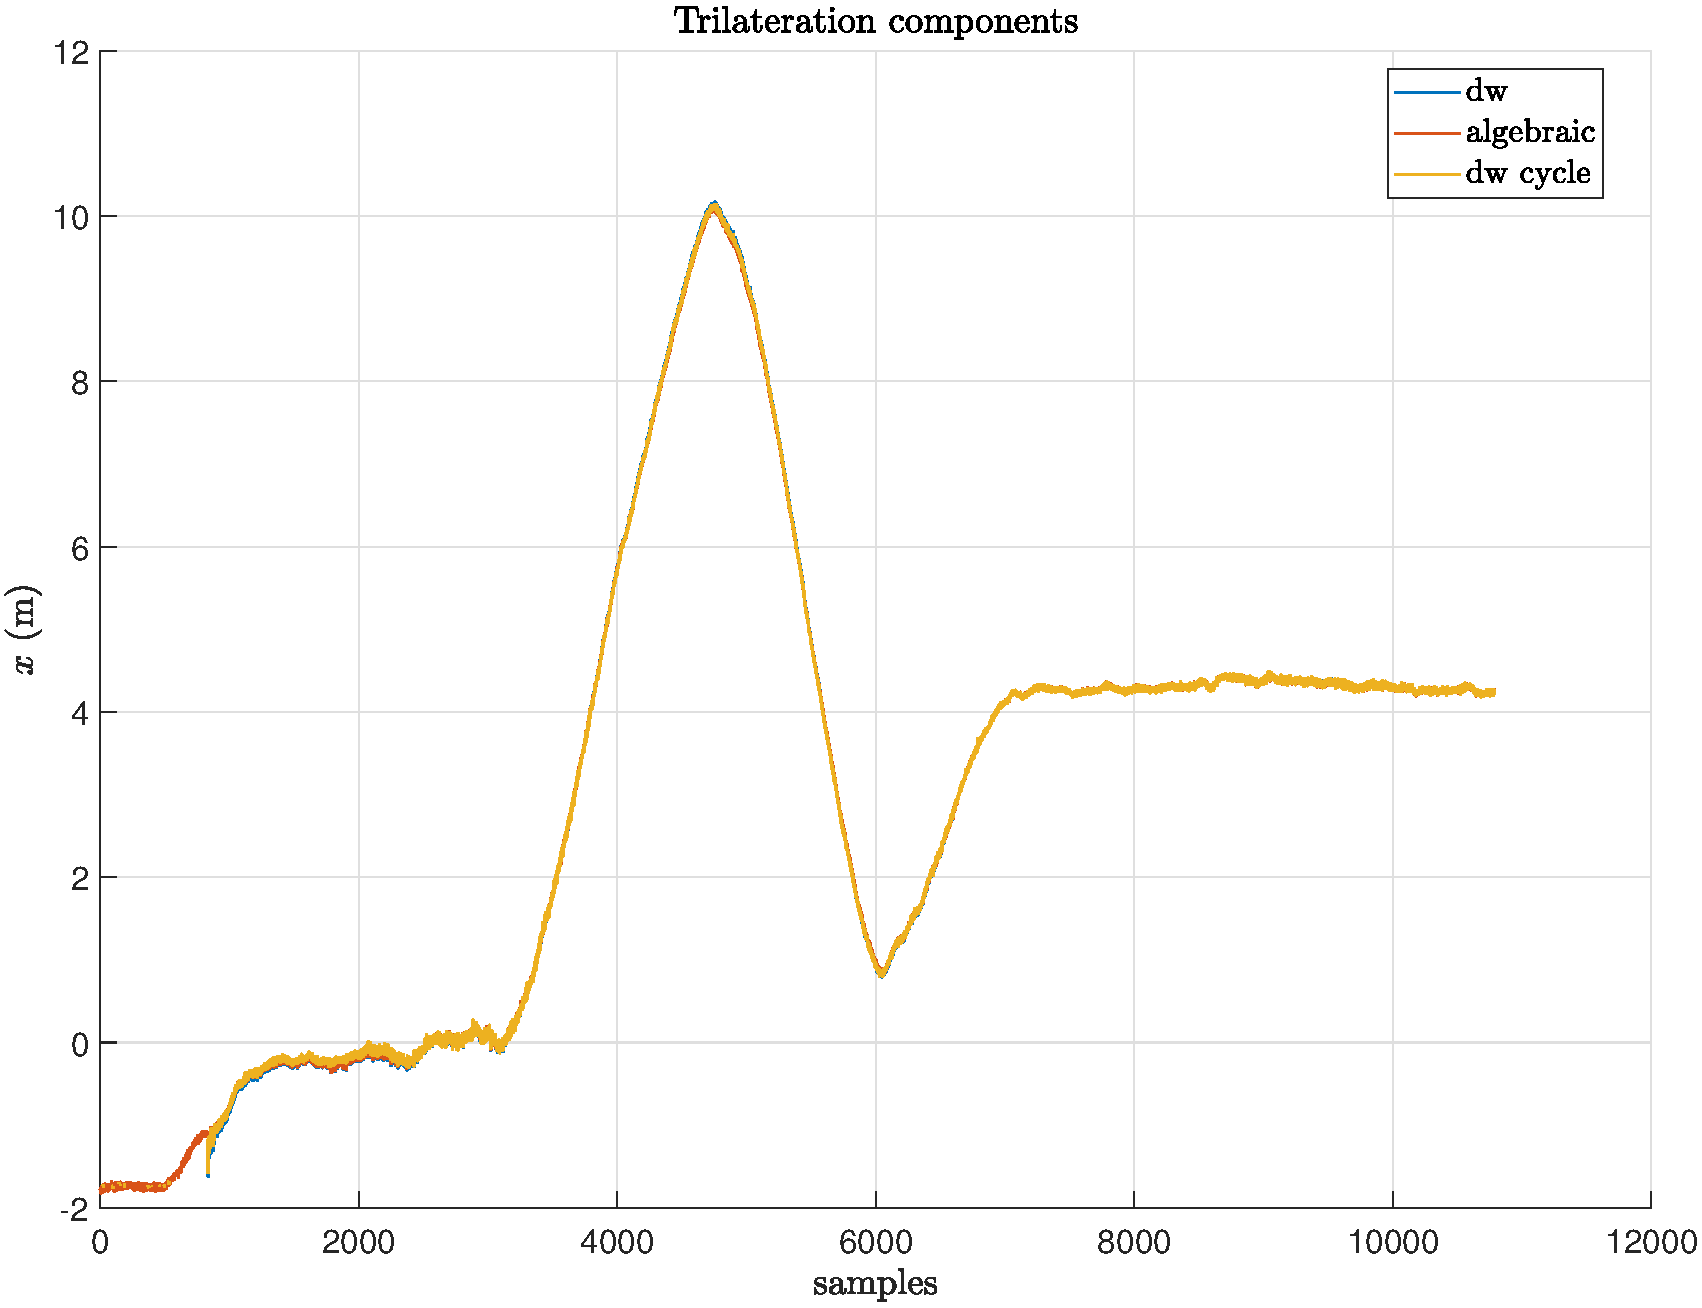
\includegraphics[height=19em]{algorithm_x.pdf}
  \end{center}
\end{frame}

\begin{frame}{Trilaterazione: confrontro tra DecaWave, DecaWave Cycle e Algebraic}
  \begin{center}
    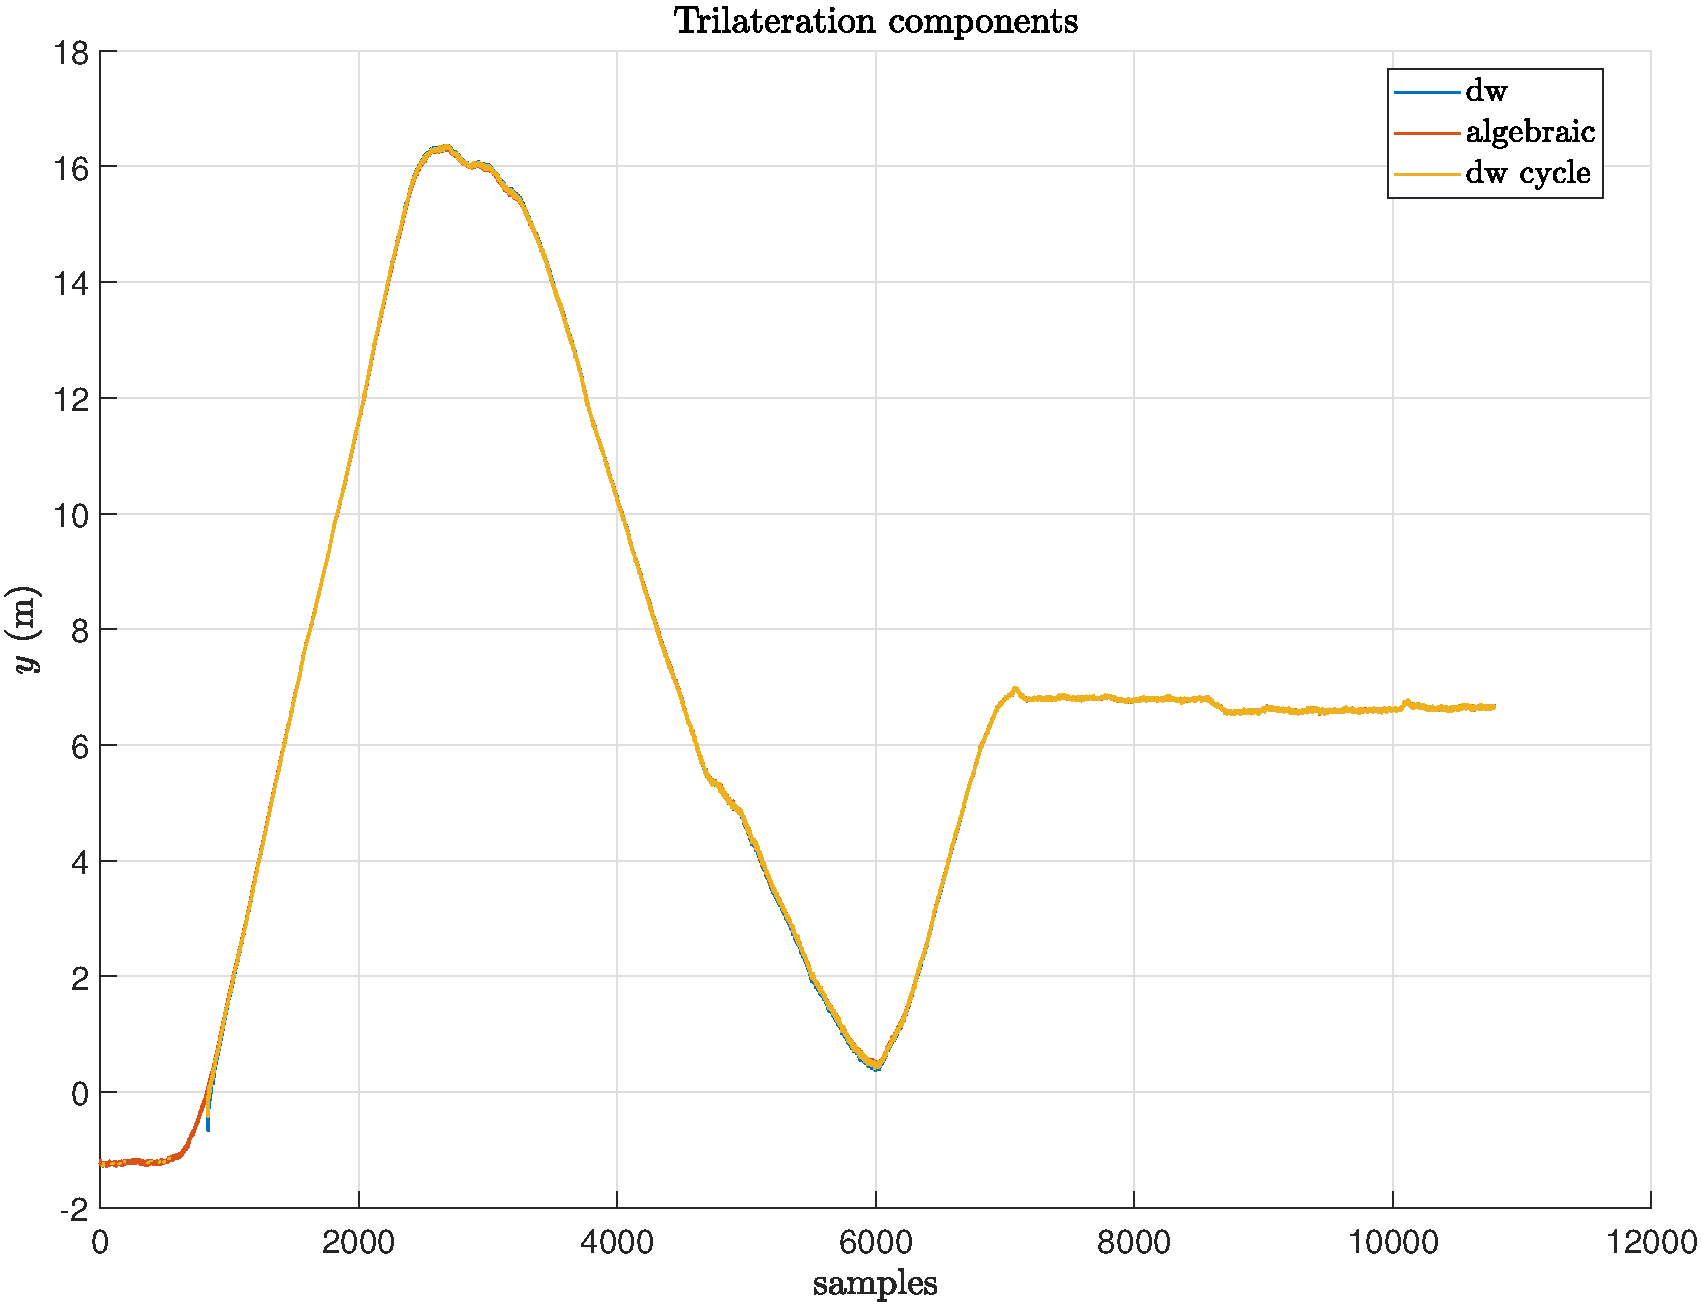
\includegraphics[height=19em]{algorithm_y.pdf}
  \end{center}
\end{frame}

\begin{frame}{Trilaterazione: confrontro tra DecaWave, DecaWave Cycle e Algebraic}
  \begin{center}
    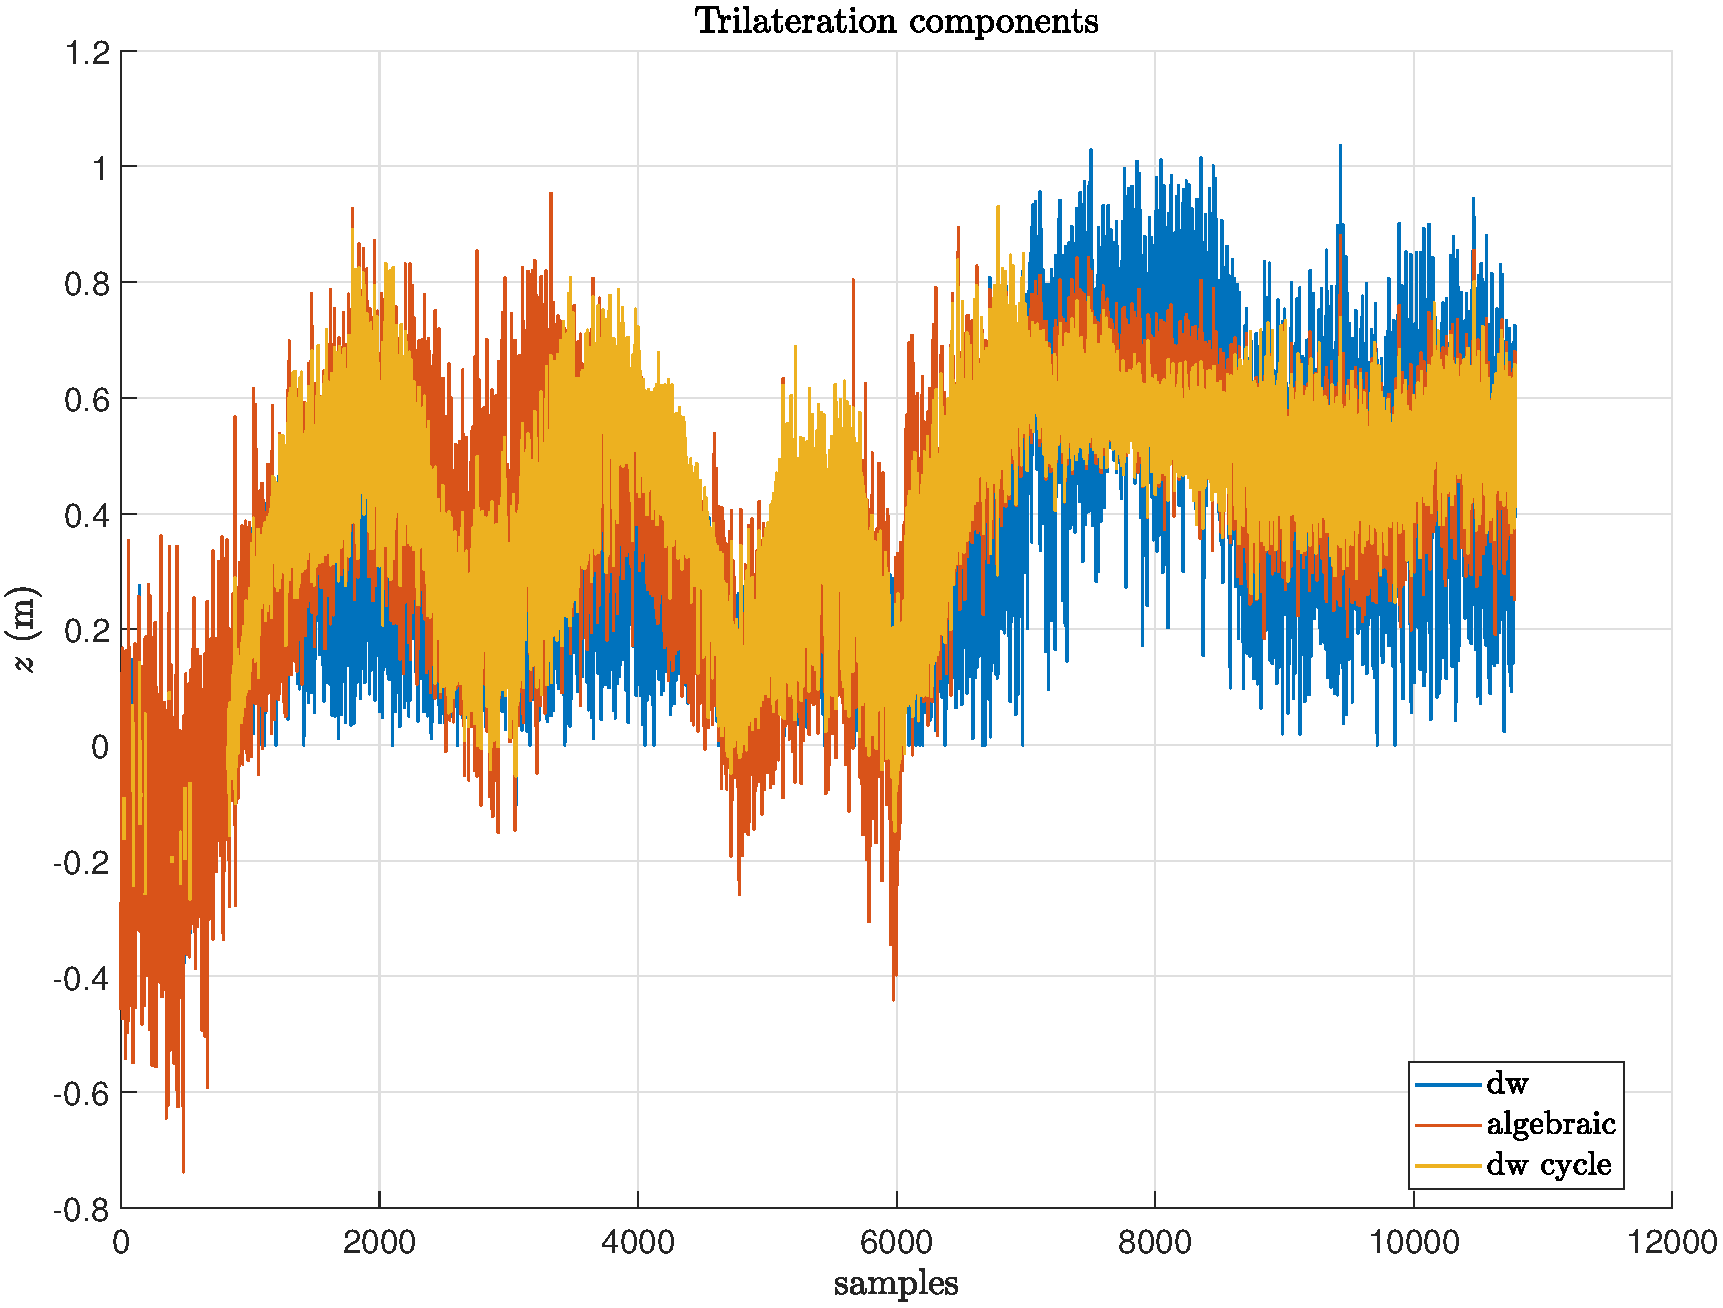
\includegraphics[height=19em]{algorithm_z.pdf}
  \end{center}
\end{frame}

\begin{frame}{Trilaterazione con due tag}
  Nel plot delle slide successiva è mostrato il risultato della trilaterazione nel caso in cui il sistema
  operi con due tag contemporaneamente (la frequenza di ranging è pari a \SI{50}{\hertz}.\\
  L'algoritmo di trilaterazione utilizzato è l'algoritmo DecaWave.
\end{frame}

\begin{frame}{Trilaterazione con due tag}
  \begin{center}
    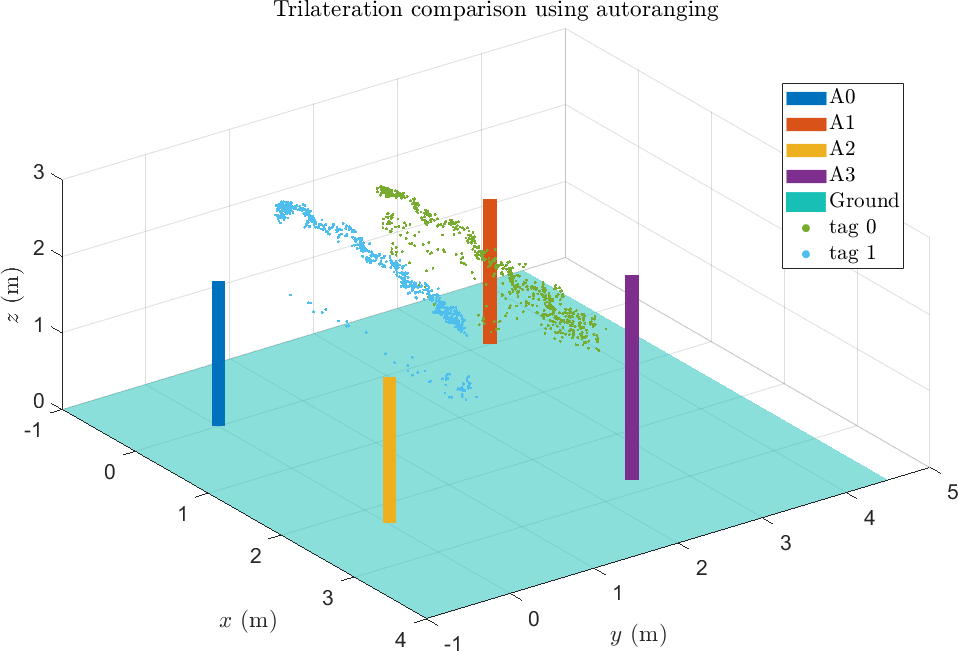
\includegraphics[height=19em]{two_tags.png}
  \end{center}
\end{frame}

\begin{frame}{Trilaterazione con due tag}
  \begin{center}
    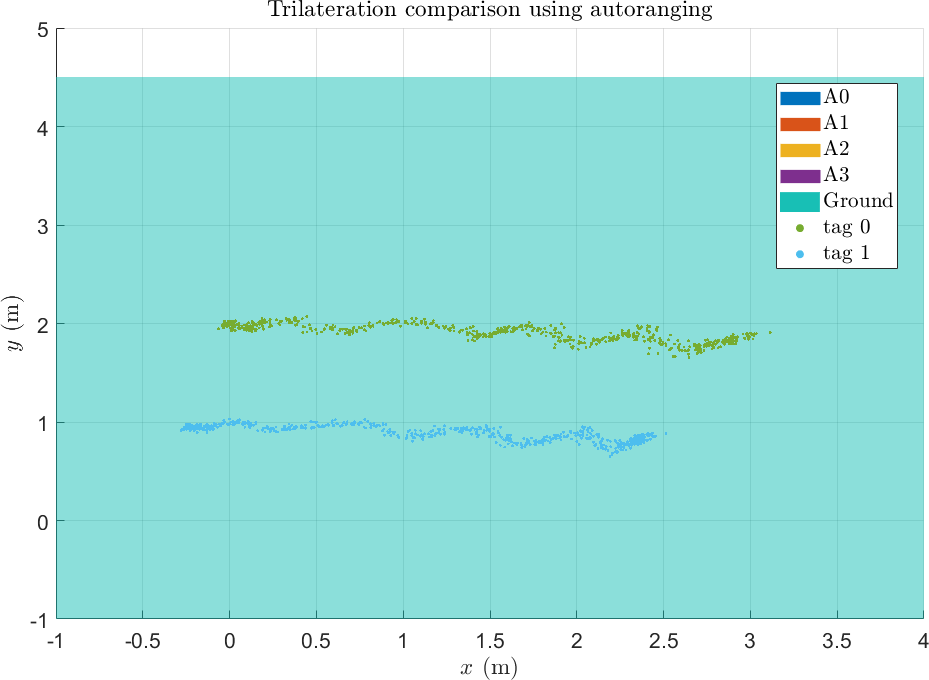
\includegraphics[height=19em]{two_tags_pianta.png}
  \end{center}
\end{frame}

\begin{frame}{Trilaterazione con due tag}
  \begin{center}
    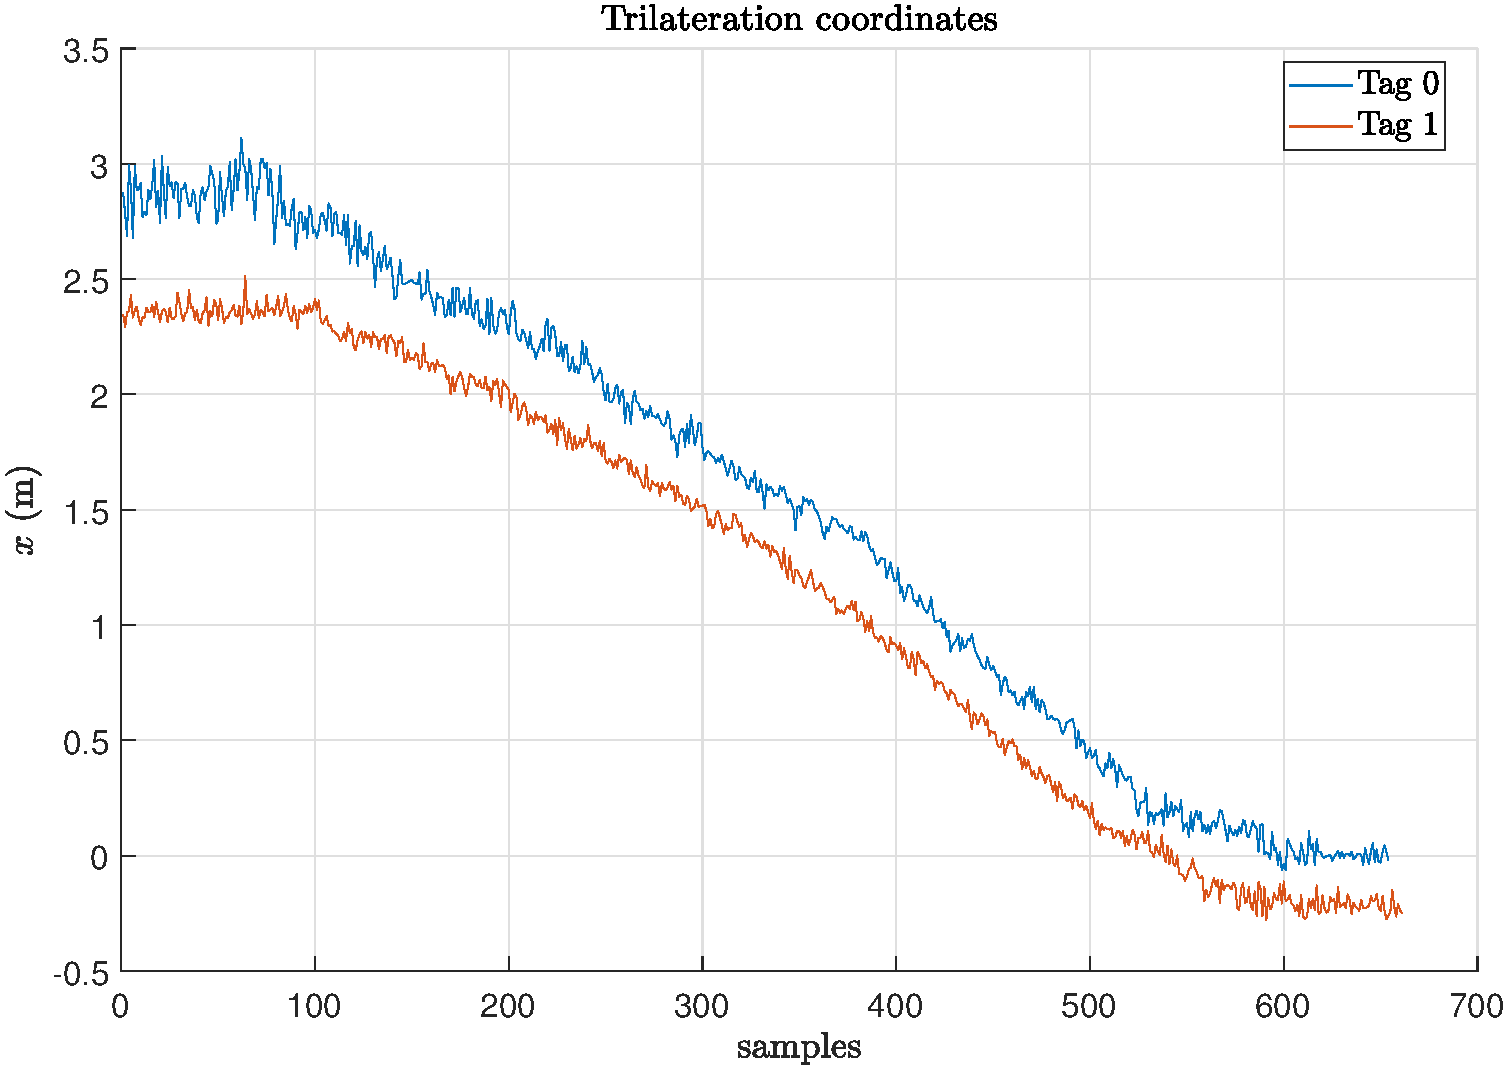
\includegraphics[height=19em]{two_tags_x}
  \end{center}
\end{frame}

\begin{frame}{Trilaterazione con due tag}
  \begin{center}
    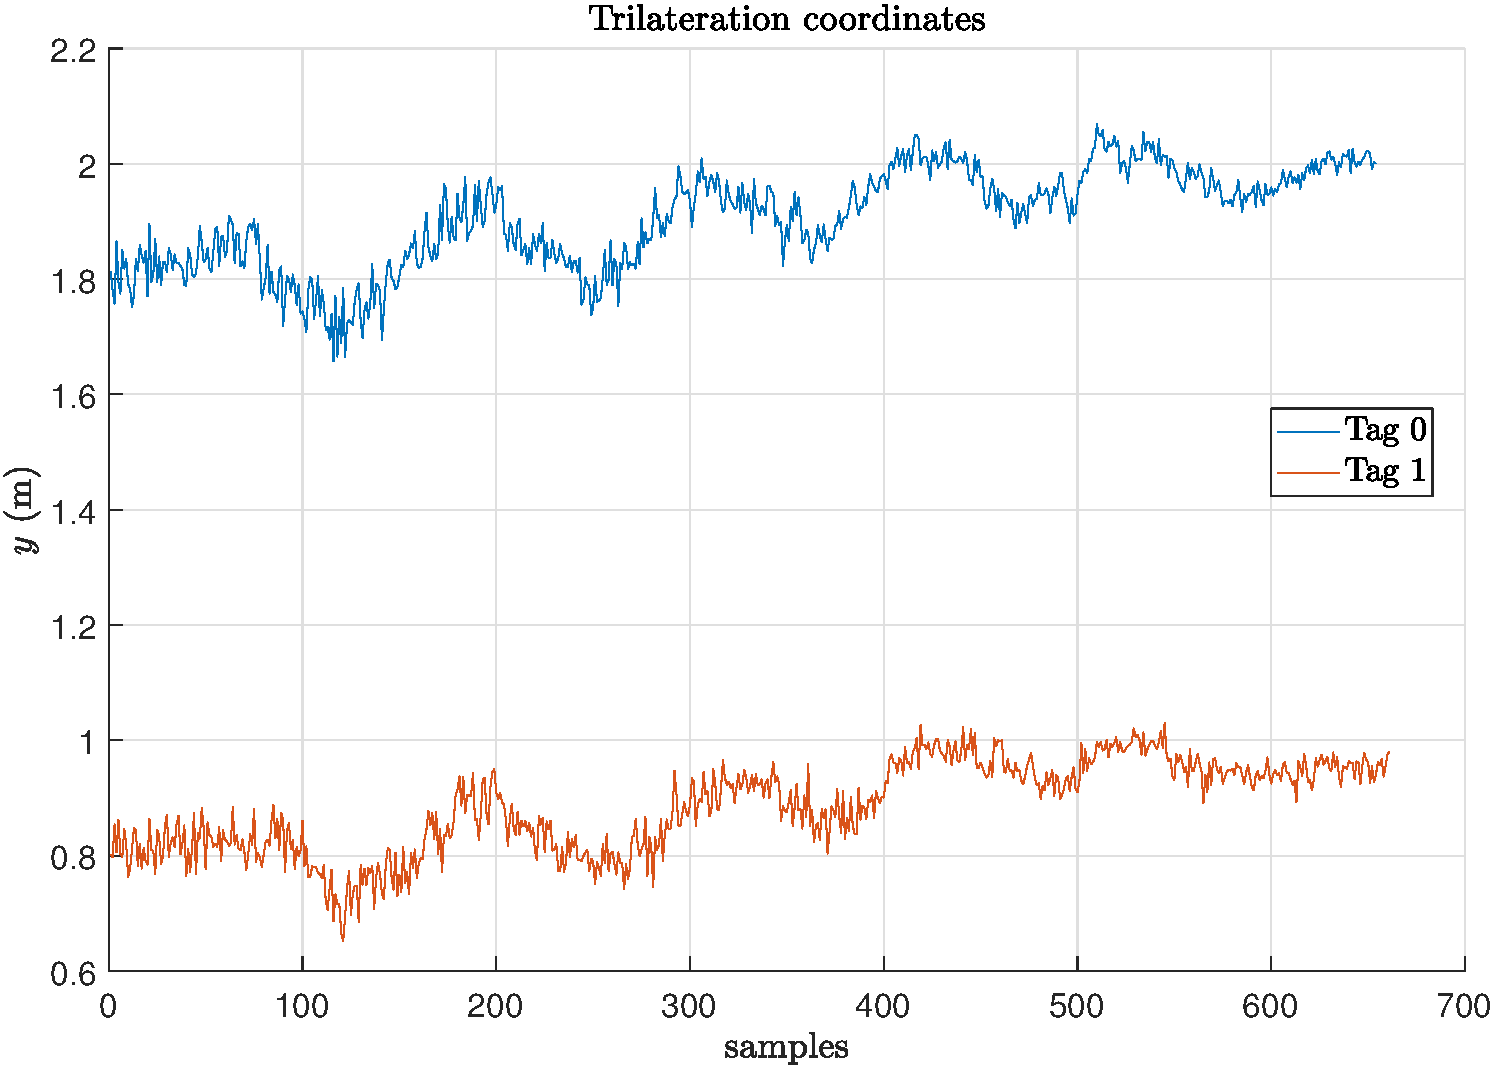
\includegraphics[height=19em]{two_tags_y}
  \end{center}
\end{frame}

\begin{frame}{Trilaterazione con due tag}
  \begin{center}
    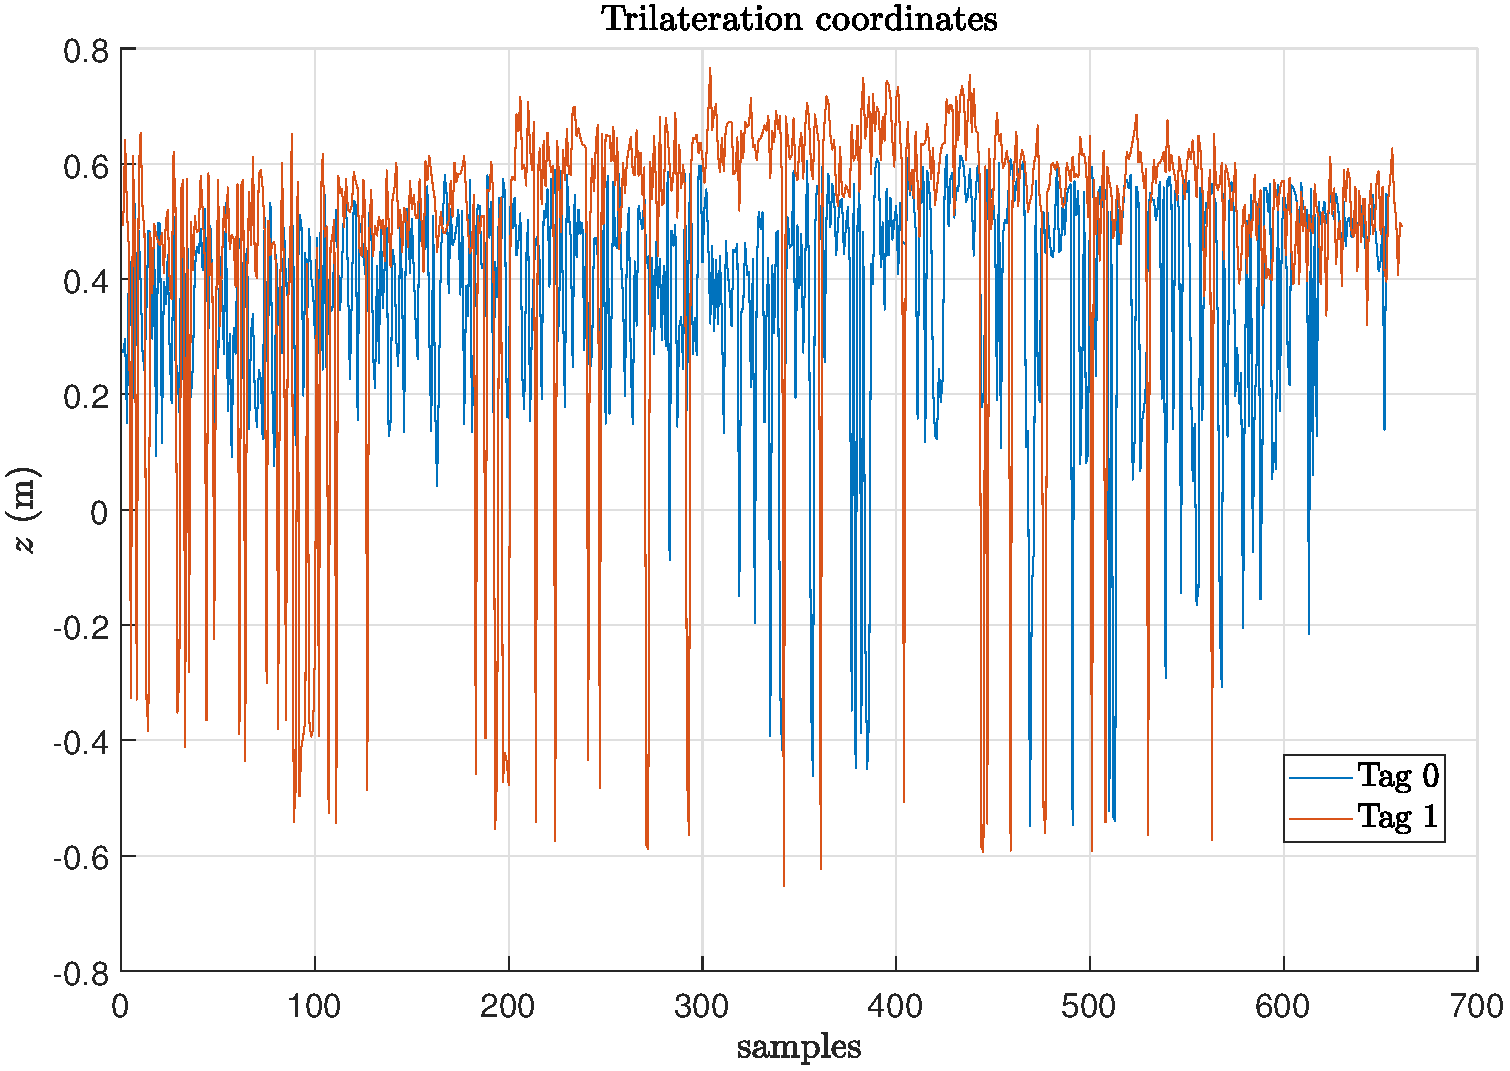
\includegraphics[height=19em]{two_tags_z}
  \end{center}
\end{frame}


